%tag:000L
%label:"prf:polterovichSurgery"
%author:JeffHicks
%name:"construction of Polterovich surgery"
%type:"proof"
%parent:prp:polterovichSurgery

 
 

There exists a \snip{standard model}{lem:straightening} of two Lagrangian submanifolds intersecting transversely at a point. Therefore, it suffices to construct a Lagrangian surgery neck for the standard intersection neighborhood $X=\CC^n$, $L_1=\RR^n$ and $L_2=\jmath\RR^n$.
We start by picking a \emph{surgery profile curve},  
\begin{align*}
      \gamma: [-R, R] \to& \CC\\
      t\mapsto& (a(t)+\jmath b(t))
\end{align*}
with the property that $a(t), b(t)$ are non-decreasing, and there exists a value $t_0$ so that 
\begin{itemize}
      \item  $\gamma(t)=t$ for $t< t_0$, and
      \item  $\gamma(t)=\jmath t$ for $t>t_0$.
\end{itemize}
We denote the are bounded between the real axis, imaginary axis, and curve $\gamma$ by $\lambda$.
An example is drawn in \cref{fig:polterovichSurgeryProfile}.
%tag:000X
%label:"fig:polterovichSurgeryProfile"
%author:JeffHicks
%name:"surgery profile"
%type:"figure"
%parent:def:polterovichSurgery
%caption:"Surgery Profile for Polterovich surgery"



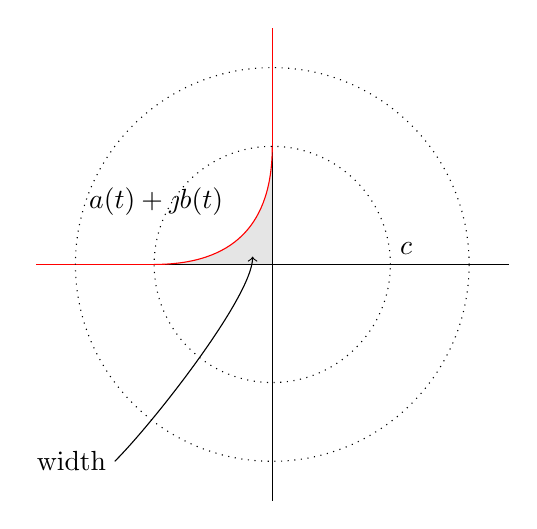
\begin{tikzpicture}

    \fill[fill=gray!20] (-1.5,0) .. controls (-0.5,0) and (-0.5,0) .. (0,0) .. controls (0,0.5) and (0,0.5) .. (0,1.5) .. controls (0,0.5) and (-0.5,0) .. (-1.5,0);
    
    \draw (0,3) -- (0,-3);
    \draw (3,0) -- (-3, 0);
    \draw[red] (-3, 0)--(-1.5,0) (0,1.5)--(0, 3);
    \draw[red] (-1.5,0) .. controls (-0.5,0) and (0,0.5) .. (0,1.5);
    \node[above left] at (-0.5,0.5) {$a(t)+\jmath b(t)$};
    \node[above right] at (1.5,0) {$c$};
    \draw[dotted]  (0,0) ellipse (1.5 and 1.5);
    \draw[dotted]  (0,0) ellipse (2.5 and 2.5);
    \draw[->] (-2,-2.5) .. controls (-1.5,-2) and (-0.25,-0.4) .. (-0.25,0.1);
    \node at (-2.55,-2.5) {width};
\end{tikzpicture}
This data provides a construction for the Lagrangian surgery neck:
\[
	L_1\#_\gamma L_2:=\left\{(\gamma(t)\cdot x_1,\ldots,  \gamma(t)\cdot x_n) \text{ such that } x_i \in \RR^n,t\in \RR, \sum_{i} x_i^2=1\right\}.
\]
Note that when $t < t_0$ this parameterizes $(\RR\setminus B_r(0))\subset \CC^n$, and when $t > t_0$ the chart parameterizes $(\jmath \RR \setminus B_r(0))\subset \CC^n$. 
Therefore, this construction satisfies the condition that the surgery Lagrangian agrees with the surgery components outside of a small neighborhood of the surgery point.
This Lagrangian has the topology of $S^{n-1}\times \RR$, which is the local model for the connect sum $\RR^n\#_0\RR^n$.


\Cref{prp:polterovichSurgery} follows by taking $L_1\#_\gamma L_2$ for any suitable choice of $\gamma$.
 